\documentclass[12pt, a4paper, oneside]{article}


\usepackage[utf8]{inputenc}
\usepackage[hidelinks]{hyperref}
\hypersetup{
    colorlinks=true,
    linkcolor=black,
    filecolor=magenta,
    urlcolor=blue,
    pdftitle={Internship Report},
    pdfpagemode=FullScreen,
}
\usepackage[none]{hyphenat}
\usepackage{pythonhighlight}
\usepackage{graphicx}
\graphicspath{{./images/}}


\title{\huge Internship Report}
\author{Mattia Evangelisti \\ s268637}
\date{June 2022}


\begin{document}

\begin{titlepage}
    \maketitle
\end{titlepage}

\tableofcontents
\clearpage\null\newpage


\newpage
\section{Summary}
During my internship experience with Ubroker, I have developed my own data mining project from scratch, developing the necessaries skills and knowledge.\\
The main objective of the project was to retrieve data about employees, company devices and their usage, and to create reports that would be useful for the company.\\
The project was developed in Python, language that I learned thanks to the constant support of my colleagues.\\
The key points of the project could be summarized as follows: data retrieval from Microsoft Azure, through the use of Microsoft Graph APIs, data manipulation, data storage in an internal database,
and the creation of reports.\\
Although I found the project to be a challenging experience, I found it to be valuable in developing my skills in Python programming, data manipulation and database management.\\


\newpage
\section{Company}
Ubroker srl was founded in 2015 with the goal of providing eco-friendly energy to their clients, without neglecting the need of a competitive price.\\
More information can be found in their \href{https://ubroker.it/}{website}.
\subsection{Mission}
The company's mission is to improve the life quality of its clients by granting them a simple management system that allows them to control their energy consumption and a cost saving service, providing 
competitive prices below the market average. Moreover, Ubroker is constantly striving to maintain the social responsibility by choosing providers who follow policies that safeguard the environment and cultures
involved in the energy distribution process.

\subsection{Market Strategy}
Ubroker is an electricity and gas provider, that collocate itself at the last link of the energy distribution chain. Their working area is indeed the sales to the final client.\\
The company sales target is the domestic market, the majority of their customers are private citizens. The most recent data report 85,000 active clients, who subscribed 52,000 electricity contracts
and 32,000 gas contracts.\\
The peculiarity of Ubroker's market strategy is the system called \emph{scelgo zero}. Each client can join the zero project though their \href{https://scelgozero.it/}{platform} and start to reduce to zero their
electricity and gas bill.\\
On their website, each client may have two options: to become a testimonial and start to zero their bills and the possibility to become an advisor of the zero project. The first option allows the clients to reduce their bill, indeed each user will receive points
every time they invite a new client and every time an invited user bring in someone else. Through this mechanism, the bill will be proportionally reduced, possibly until zero.
On the other hand, by choosing the second options, a user may become an external advisor, whose role will be to sell contracts to new potential clients, earning a commission for each new subscription. 
Moreover, those external partners will have access to a wide range of training courses, that can be chosen and followed on the platform.

\newpage
\subsection{Economic Growth}
Ubroker was founded in 2015 and since then, thanks to the innovative market strategy and the strong digitalization of all the services, the company has been able to grow rapidly. Thanks to those characteristics,
they were able to achieve incredible goals, such as a total of 170000 clients and over 2 million issued invoices. Moreover, the company has recently gained a Microsoft partnership.

\subsection{Working environment}
The company currently employs about 50 people, divided in various departments, such as sales, marketing, IT, legal, accounting, etc.\\
The main office is located in the city of Collegno, in the metropolitan area of Turin and, at the moment is composed of one building, but they will be able to expand their space in a second build, within the next
few months. Moreover, the company is still granting to the employees the possibility of working remotely, through the use of devices provided by the company itself.

\subsection{IT department}
Being a computer engineering student, I spent most of my internship in the IT department, which is composed of a team of 8 people. The main goal of this department is the software development, 
for both internal and external use.\\ 
The team covers all the aspects of a software life, from the development of the software itself, including both front-end and back-end development, to the integration and the maintenance of the software with the company's 
infrastructure.\\
The main projects of the IT department are: \emph{Piattaforma Zero}, which was described before, several web applications used by the other departments and an internal system for the management of the company's contracts.\\
All the software are developed using the Docker technology, which allows to create a containerized environment, in which the software can be developed, installed and run. The front-end developing is mostly done
using the JavaScript framework Angular, on the other hand, the back-end developers deals with PHP framework Laminas and PostgreSQL databases.\\
Moreover, I found fascinating how the whole infrastructure is cloud based. The company make indeed an intense use the Azure cloud, which is a cloud computing platform owned by Microsoft, that allows
to have storage and virtual machines in the cloud. Ubroker uses about 60 virtual machines and over 6 TB of storage on the Azure platform. Thanks to this intense use of this service, the company is recently
become a Microsoft partner.\\
My role in the department was to create a software able to retrieve data about employees, company devices and their usage, and to create reports that would be useful for the company.

\newpage
\section{Project}
The project can be summarized in 4 main parts:
\begin{itemize}
    \item Data retrieval from Microsoft Azure, through the use of Microsoft Graph APIs.
    \item Data cleaning and manipulation.
    \item Data storage in an internal database.
    \item Report creation using Power Bi.
\end{itemize}
\subsection{Used technologies}
The project was entirely written in Python 3.9 programming language and the following libraries were used:
\begin{verbatim}
    colorama==0.4.4
    jsonschema==4.4.0
    msal==1.17.0
    pandas==1.4.2   
    psycopg2==2.9.3
    requests==2.27.1
    tabulate==0.8.9
\end{verbatim}
For the database management it was chosen to use PostgreSQL, as long with BDeaver, which is a SQL client software application and a database administration tool.\\
The project was developed using the GIT version control system, integrated with the hosting system GitHub. These two tools allow to store, modify and share the project's code, as well as to keep a records
of the activities and modifications done.\\
The data retrieving was carried out thanks to the Microsoft Graph API, which is a REST API that allows to retrieve data from Microsoft Azure.\\
Finally, the report creation was done using Power Bi, a Microsoft tool that allows to create reports in a simple and intuitive way.

\newpage
\subsection{Standards}
The whole Python coding part of the project was written following the \href{https://peps.python.org/pep-0008/}{PEP8} Style Guide for Python Code.
This guide gives coding conventions for the Python code comprising the standard library in the main Python distribution.\\
The application was developed from scratch, so I had to organize the files in order to maintain a precise schema. In particular mine was a command-line application composed by a main file, called \emph{console.py}
and several other internal packages. Following the \href{https://realpython.com/python-application-layouts/}{standard layout}, I divided all my files into subfolders, each one containing packages divided with
respect to their use and their functionality.\\
Throughout the developing of my project, I made an extensive use of the Docker technology, which allowed me to create a containerized environment, isolated from the rest of the system,
in which the software was developed, tested and run.

\subsection{Training}
During my internship experience I was able to learn several new technologies, I indeed spent the first week of my internship learning everything I would have needed for the developing of the project.\\
First I had to learn Python programming language, to which I was totally new. This task was carried out following different tutorials and thanks to the constant support of company tutor, who assisted me in
my training. The learning of this language was not very difficult, since, thanks to the courses I followed, I already had a strong coding background.\\
Then I start to discover the API world, particularly I had to learn how to make REST HTTP request to an endpoint in Python. Fortunately, I had already studied the basics of the HTTP protocol and the REST architecture
during the course of \emph{Introduction to databases}, so I only had to adapt my previous knowledge to the Python language.\\
Finally yet importantly, I learned, how to manage my progresses using the version control system GIT. It was the first time I used it in a working environment, but thanks to the course of \emph{Object oriented programming},
I already had experience with the SVN version control system.

\newpage
\subsection{Console menu}
The main file and the only one which was effectively run, is the \emph{console.py} file. This file is composed by a main menu, which allows to choose the desired command.\\
The menu allows the user to choose which command to run or to open a help menu, which provide the user with information about the available commands and their usage. The selected command has to be passed as a
parameter when the script is run, some commands may accept optional parameters as indicated in the help menu. If no command is specified, the default action is to open the help menu.
\begin{figure}[h]
    \centering
    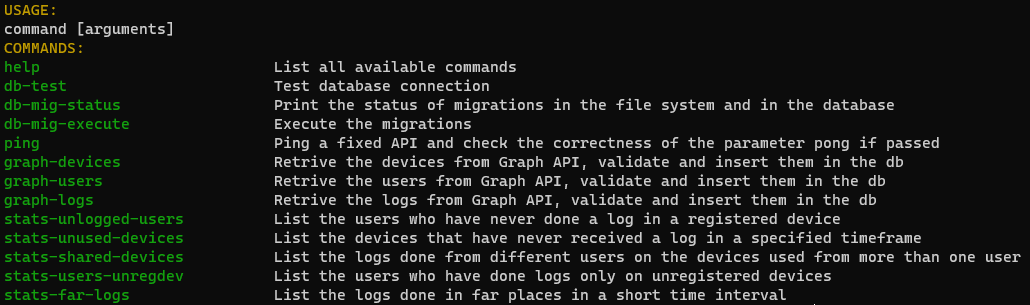
\includegraphics[width=\textwidth, height=7cm]{help-menu.png}
    \caption{help menu}
\end{figure}\\
Summing up, the main role of the console is to import all the required packages and execute the commands, through all the function contained in the other files.

\subsection{Configuration}
The parameters needed in the project, such as database information, API URLs, JSON files and other data files, are stored in the \emph{config.ini} file. This allows the user to have a much more clear
overview of the possibility to change the information based on the current needs.\\
On the other hand this data are not directly contained in the Python code, so they need to be retrieved. The \emph{ConfigParser} package comes in our help, allowing as to retrieve the data from the config file
and return them in any Python function.
\begin{python}
    def get_url():
        parser = ConfigParser()
        parser.read("config.ini")
        url = parser.get('ping', 'url')
        return url
\end{python}
The above code is an example of how the configuration function works. In the example, the parameter \emph{url} is retrieved from the section \emph{ping} of the \emph{config.ini} file.


\subsection{Database Connection}

\end{document}